\section{语言基础}

\subsection{分层学习方案}

\textit{“工欲善其事，必先利其器” —— 掌握 C++ 是算法竞赛的第一步}

\subsubsection{校内必修课程情况}

\begin{figure}[H]
	\centering
	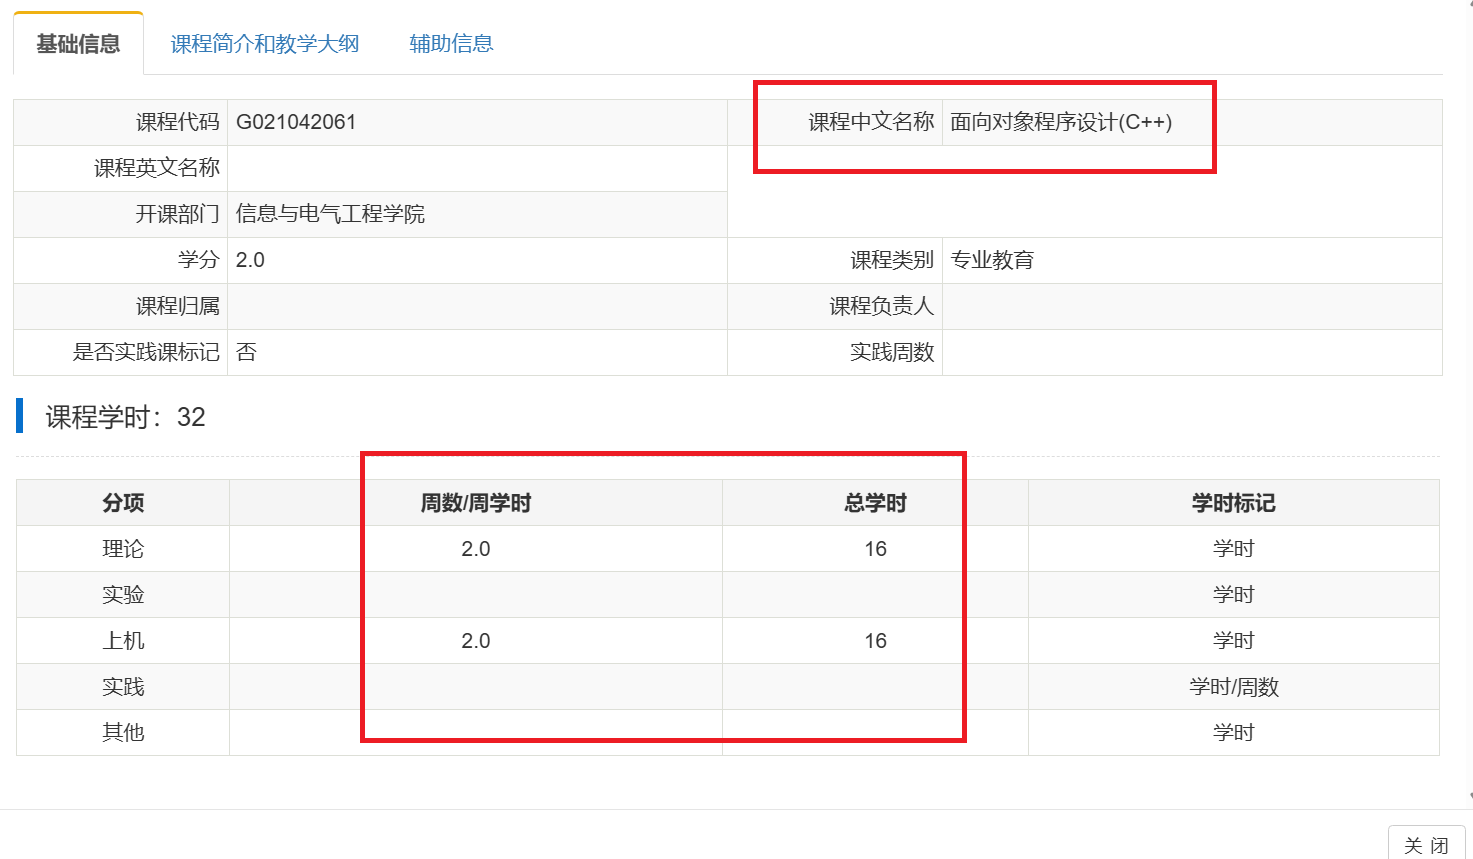
\includegraphics[width=0.9\linewidth]{figure/cpp-course}
	\caption{面向对象程序设计(C++)课程基础信息}
	\label{fig:cpp-course}
\end{figure}


\subsubsection{有语言基础}
\textbf{目标：} 从“面向过程编程(C语言)”转向“面向竞赛编程”，熟悉 C++ STL 常用容器及其操作。


\text{STL学习教程：}\href{https://www.runoob.com/cplusplus/cpp-stl-tutorial.html}{C++ STL 教程},\href{https://blog.csdn.net/2203_75327677/article/details/136080887}{C++ STL 教程}

\begin{enumerate}
    \item \textbf{重点任务：}
        \begin{enumerate}
            \item 熟练使用算法竞赛常用的STL容器.
            \item 掌握STL容器封装的算法.
            \item 学习 C++11$\sim$C++17的新特性（如 \texttt{auto}, \texttt{range-based for loop}，\texttt{结构化绑定}）。
        \end{enumerate}
    \item \textbf{练习建议：} 查漏补缺，完成“牛客新手130题”后续的算法入门部分和AcWing的算法基础题集.\footnote{AcWing算法基础课笔记1:\url{https://www.cnblogs.com/harder-summer/articles/18832373}}\footnote{AcWing算法基础课笔记2\url{https://www.cnblogs.com/littlehb/p/15393332.html}}
\end{enumerate}

\subsubsection{无语言基础}
\textbf{目标：} 从零开始，掌握 C++ 的核心语法，达到能独立编写逻辑程序的水平。
\begin{enumerate}
    \item \textbf{重点任务：}
        \begin{enumerate}
            \item 环境搭建：安装 CLion / Dev-C++ / VS Code。
            \item 基础语法：熟悉并掌握C++风格的变量、数据类型、输入输出 (\texttt{cin}/\texttt{cout})。
            \item 控制结构：\texttt{if-else}, \texttt{for}, \texttt{while} 循环。
            \item 数组与函数：一维/二维数组、递归函数基础。
            \item 进阶基础：结构体 (\texttt{struct})、指针（仅需理解基本概念）。
        \end{enumerate}
    \item \textbf{练习建议：} 尽快完成“牛客网新手130题”和学校E2E平台的基础题库。
\end{enumerate}

\newpage


\section{第一周练习安排(初定)}

\textbf{主线计划安排如下:}

\subsection{有语言基础}

\subsubsection{完成牛客算法入门相关题目:}

题目链接:\url{https://www.nowcoder.com/exam/oj?page=1&tab=%E7%AE%97%E6%B3%95%E5%AD%A6%E4%B9%A0%E7%AF%87&topicId=385}

首周计划练习的题号为\texttt{BGN1$\sim$BGN40}

除此之外,每天还会安排一些其他题目练习，\textbf{将需要讲解的题目进行征集},晚上安排讲解.

\subsubsection{完成AcWing相关题目:}

题号见:\url{https://www.cnblogs.com/littlehb/p/15393332.html}

除此之外，每天还会安排一些其他题目练习



\subsection{无语言基础}


\subsubsection{完成AcWing 语法基础课程的题目:}

题号如下:

{
AcWing 1. A + B

AcWing 608. 差

AcWing 604. 圆的面积

AcWing 606. 平均数1

AcWing 609. 工资

AcWing 615. 油耗

AcWing 616. 两点间的距离

AcWing 653. 钞票

AcWing 654. 时间转换

AcWing 605. 简单乘积

AcWing 611. 简单计算

AcWing 612. 球的体积

AcWing 613. 面积

AcWing 607. 平均数2

AcWing 610. 工资和奖金

AcWing 614. 最大值

AcWing 617. 距离

AcWing 618. 燃料消耗

AcWing 656. 钞票和硬币

AcWing 655. 天数转换

}

\textbf{题解及笔记}：\url{https://www.codeleading.com/article/71505239127/#AcWing_655__462}

\subsubsection{完成牛客网C++入门相关练习}

题目链接:\url{https://www.nowcoder.com/exam/oj?page=1&tab=%E8%AF%AD%E8%A8%80%E5%AD%A6%E4%B9%A0%E7%AF%87&topicId=225}

\textbf{\color{red} 这两部分的内容较为基础,不再安排专门讲解,可以结合题解和合理使用AI工具学习,确保基础内容完全掌握.
}

\subsection{自行安排}

\textbf{线上比赛:}
\begin{enumerate}
	\item 每周六晚8点$\sim$9点40,AtCoder平台ABC
	\item 每周日晚7点,牛客竞赛-周赛
\end{enumerate}



完成上述计划,如还有额外精力,推荐自行学习数据结构的内容,并且练习洛谷和AcWing的其他内容.

